% Required packages: tikz, xcolor, amsmath
% Required TikZ libraries: none
% Target width: 161 mm
% Minimum text size: 7 pt at final reproduction
% Colour/greyscale intent: dark ink and one restrained accent; orientations and direct labels are redundant.
\begingroup
\definecolor{runInk}{RGB}{38,44,51}%
\definecolor{runQuiet}{RGB}{95,104,109}%
\definecolor{runAccent}{RGB}{146,65,36}%
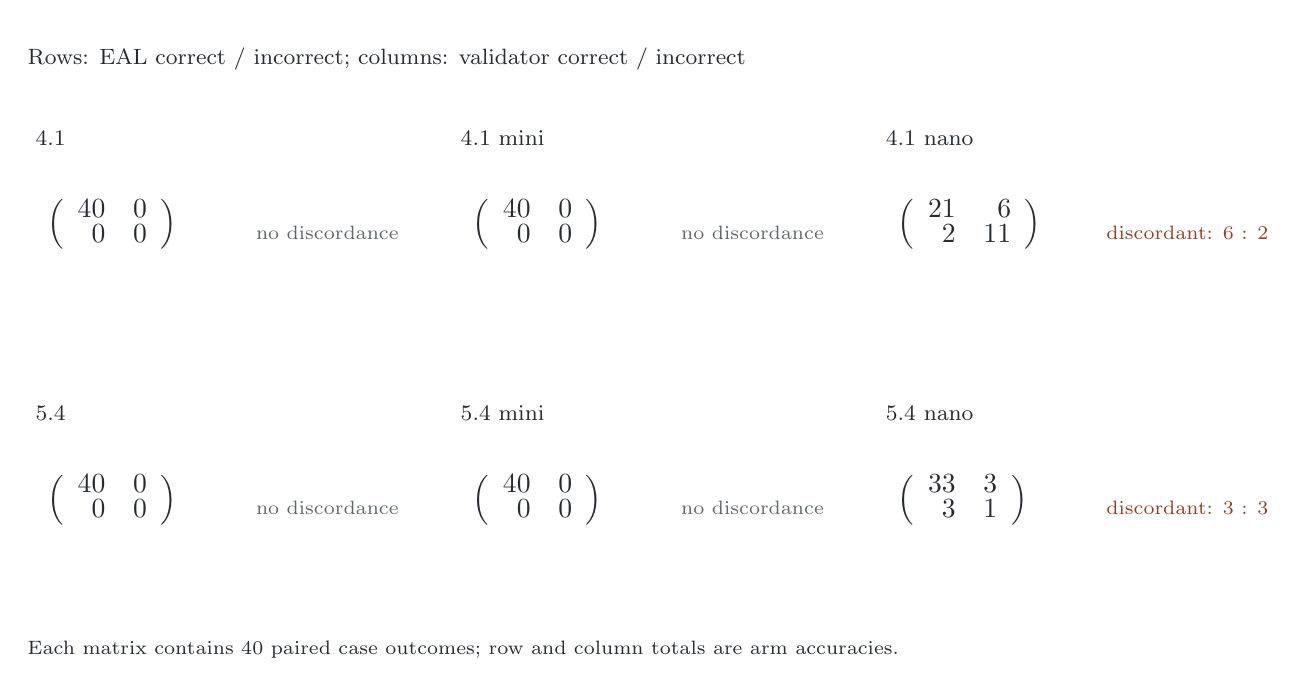
\begin{tikzpicture}[x=1mm,y=1mm,inner sep=0pt,outer sep=0pt]
\useasboundingbox (0,0) rectangle (160,81);
\node[anchor=west,text=runInk,font=\fontsize{7.8}{9}\selectfont] at (0.000,77.000) {Rows: EAL correct / incorrect; columns: validator correct / incorrect};
\node[anchor=west,text=runInk,font=\fontsize{8}{9}\selectfont] at (1.000,67.000) {4.1};
\node[anchor=west,text=runInk,font=\fontsize{10}{9}\selectfont] at (2.500,56.000) {$\left(\begin{array}{rr}40&0\\0&0\end{array}\right)$};
\node[anchor=west,text=runQuiet,font=\fontsize{7}{9}\selectfont] at (29.000,55.000) {no discordance};
\node[anchor=west,text=runInk,font=\fontsize{8}{9}\selectfont] at (55.000,67.000) {4.1 mini};
\node[anchor=west,text=runInk,font=\fontsize{10}{9}\selectfont] at (56.500,56.000) {$\left(\begin{array}{rr}40&0\\0&0\end{array}\right)$};
\node[anchor=west,text=runQuiet,font=\fontsize{7}{9}\selectfont] at (83.000,55.000) {no discordance};
\node[anchor=west,text=runInk,font=\fontsize{8}{9}\selectfont] at (109.000,67.000) {4.1 nano};
\node[anchor=west,text=runInk,font=\fontsize{10}{9}\selectfont] at (110.500,56.000) {$\left(\begin{array}{rr}21&6\\2&11\end{array}\right)$};
\node[anchor=west,text=runAccent,font=\fontsize{7}{9}\selectfont] at (137.000,55.000) {discordant: 6 : 2};
\node[anchor=west,text=runInk,font=\fontsize{8}{9}\selectfont] at (1.000,32.000) {5.4};
\node[anchor=west,text=runInk,font=\fontsize{10}{9}\selectfont] at (2.500,21.000) {$\left(\begin{array}{rr}40&0\\0&0\end{array}\right)$};
\node[anchor=west,text=runQuiet,font=\fontsize{7}{9}\selectfont] at (29.000,20.000) {no discordance};
\node[anchor=west,text=runInk,font=\fontsize{8}{9}\selectfont] at (55.000,32.000) {5.4 mini};
\node[anchor=west,text=runInk,font=\fontsize{10}{9}\selectfont] at (56.500,21.000) {$\left(\begin{array}{rr}40&0\\0&0\end{array}\right)$};
\node[anchor=west,text=runQuiet,font=\fontsize{7}{9}\selectfont] at (83.000,20.000) {no discordance};
\node[anchor=west,text=runInk,font=\fontsize{8}{9}\selectfont] at (109.000,32.000) {5.4 nano};
\node[anchor=west,text=runInk,font=\fontsize{10}{9}\selectfont] at (110.500,21.000) {$\left(\begin{array}{rr}33&3\\3&1\end{array}\right)$};
\node[anchor=west,text=runAccent,font=\fontsize{7}{9}\selectfont] at (137.000,20.000) {discordant: 3 : 3};
\node[anchor=west,text=runInk,font=\fontsize{7.2}{9}\selectfont] at (0.000,2.000) {Each matrix contains 40 paired case outcomes; row and column totals are arm accuracies.};
\end{tikzpicture}
\endgroup\ignorespaces
